\problemname{\problemyamlname}

\illustration{0.2}{bomb.jpg}{
    CC BY-SA 4.0 by goff.brian on \href{https://www.vecteezy.com/vector-art/552160-bomb}{Vecteezy}
}

Oh non, il y a une bombe dans votre cuisine ! Vous devez la désamorcer avant qu'elle n'explose. Pour ce faire, vous devez résoudre un puzzle.
Vous disposez d'une grille avec $n$ lignes et $m$ colonnes. Chaque case contient une couleur. Chaque ligne contient deux flèches, une qui pointe vers la gauche, l'autre vers la droite.
Quand on appuie sur la flèche de droite, toutes les couleurs de la ligne sont déplacées d'une case vers la droite, et quand on appuie sur celle de gauche, elles sont déplacées d'une case vers la gauche.
Les lignes sont cycliques, donc si une couleur sort d'un côté de la ligne, elle rentre de l'autre côté.

Votre but est de trouver deux lignes qui sont égales après avoir entré une séquence de flèches. Si vous trouvez deux lignes qui sont égales, alors vous avez désamorcé la bombe. Si vous n'arrivez pas à trouver deux lignes qui sont égales, alors la bombe explose !

\begin{figure}[H]
    \centering
    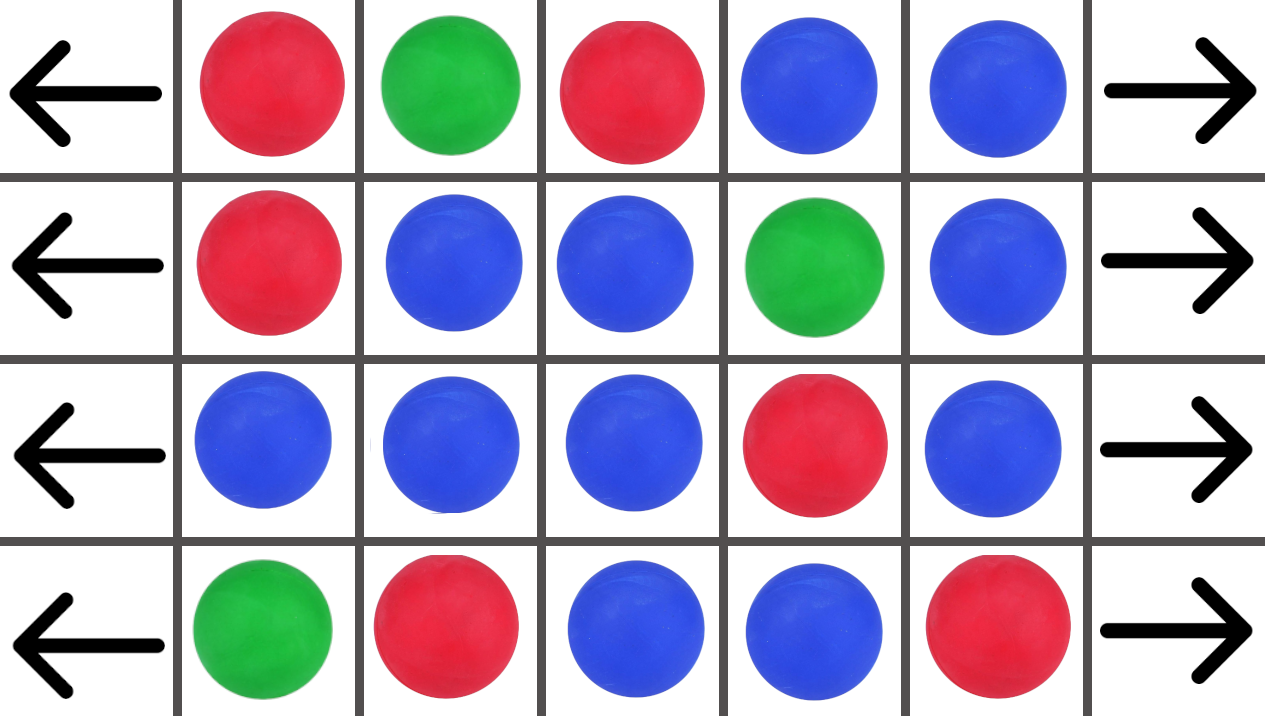
\includegraphics[width=0.5\textwidth]{illustration.png}
    \caption{Illustration de l'exemple 1}
\end{figure}

\begin{Input}
    L'entrée consiste en :
    \begin{itemize}
        \item Une ligne avec deux entiers $n$ et $m$ ($0\leq n,m \leq 10^4$), respectivement le nombre de lignes et le nombre de colonnes dans la grille,
        \item $n$ lignes, chacune contenant une chaîne de caractères de longueur $m$. Le $j$-ème caractère de la $i$-ème ligne est $a_{i,j}$, la couleur de la cellule $(i,j)$.
    \end{itemize}
    Il est garanti que $a_{i,j}$ est une lettre de l'alphabet \textbf{majuscule ou minuscule}.\\
    Il est aussi garanti que $n \times m \leq 5 \times 10^5$.
\end{Input}

\begin{Output}
    L'indice des deux lignes qui sont égales en ordre croissant. S'il y a plusieurs paires, affichez celle qui a la plus petit premier indice. Si deux paires ont le même premier indice, affichez celle qui a le plus petit deuxième indice. Si vous ne trouvez pas deux lignes qui sont égales, affichez \texttt{BOOM!}.
\end{Output}
